\newpage
\noindent
\textbf{Beispiel 2} \\ \\
a)\\ \\
Dieses System besitzt folgende Freiheitsgrade
\[
	\textbf{q}^T = \begin{bmatrix}
		x_w & \varphi_1 & \varphi_2 & l_2
	\end{bmatrix}
\]
b)\\ \\
Die jeweiligen Ortsvektoren zu den Schwerpunkten lauten
\begin{align*}	
	\textbf{r}_W &= \begin{bmatrix}
		x_W \\
		0
	\end{bmatrix}
	\\
	\textbf{r}_{S1} &= \begin{bmatrix}
		x_w + \frac{l_1}{2}\sin(\varphi_1) \\
		-\frac{l_a}{2}\cos(\varphi_1)
	\end{bmatrix}
	\\
	\textbf{r}_M &= \begin{bmatrix}
		x_W + l_1\sin(\varphi_1) + l_2\sin(\varphi_2) \\
		-l_1\cos(\varphi_1) - l_2\cos(\varphi_2)
	\end{bmatrix}
\end{align*}
c)\\ \\
Die entsprechenden Geschwindigkeiten und Winkelgeschwindigkeiten der Schwerpunkte lauten
\begin{align*}
	\textbf{v}_W = \begin{bmatrix}
		\dot{x}_W \\
		0
	\end{bmatrix}
	\quad&,\quad
	\omega_W = 0
	\\
	\textbf{v}_{S1} = \begin{bmatrix}
		\dot{x}_W  +\frac{l_1}{2}\cos(\varphi_1)\dot{\varphi}_1 \\
		\frac{l_1}{2}\sin(\varphi_1)\dot{\varphi}_1
	\end{bmatrix}
	\quad&,\quad
	\omega_{S1} = \dot{\varphi}_1
	\\
	\textbf{v}_M = \begin{bmatrix}
		\dot{x}_W + l_1\cos(\varphi_1)\dot{\varphi}_1 + \dot{l}_2\sin(\varphi_2) + l_2\cos(\varphi_2)\dot{\varphi}_2 \\
		l_1\sin(\varphi_1)\dot{\varphi}_1 - \dot{l}_2\cos(\varphi_2) + l_2\sin(\varphi_2)\dot{\varphi}_2
	\end{bmatrix}
	\quad&,\quad
	\omega_M = \dot{\varphi}_2
\end{align*}
Die kinetischen Teilenergien des Systems lauten
\begin{align*}
	T_t &= \frac{1}{2}\textbf{v}^T_w\textbf{v}_W m_W + \frac{1}{2}\textbf{v}^T_{S1}\textbf{v}_{S1}m_1 + \frac{1}{2}\textbf{v}^T_M\textbf{v}_Mm_M \\
	T_r &= \frac{1}{2} \omega_1^2J_1
\end{align*}
Damit lautet die gesamte kinetische Energie des Systems
\[
	T = T_t + T_r
\]
\newpage
\noindent
d)\\ \\
Die potentielle Energie dieses Systems setzt sich aus der zusammen die in dem Stab + Masse und der in der Feder gespeichert wird zusammen. Diese beiden Teilenergien lauten
\begin{align*}
	V_m &= -m_1g\frac{l_1}{2}\cos(\varphi_1) - m_Mg\left(l_1\cos(\varphi_1) + l_2\cos(\varphi_2)\right) \\
	V_F &= \int_{x_0}^{x_W}F_F(\tilde{x})\,\text{d}\tilde{x} \\
		&= \frac{1}{2}c_1(x_W - x_0)^2 + \frac{1}{4}c_2(x_W - x_0)^4
\end{align*}
Somit ergibt sich für die gesamte potentielle Energie 
\[
	V = V_M + V_F
\]
f)\\ \\
Der Vektor für die generalisierten Kräfte setzt sich aus zwei Teilen zusammen. Den für den Waagen und den für die Punktmasse.
Für den Waagen gilt
\begin{align*}
	\textbf{F}_{an} = \begin{bmatrix}
		F_{an} \\
		0
	\end{bmatrix}
	\quad,\quad
	\textbf{r}_{an} = \begin{bmatrix}
		x_W \\
		0
	\end{bmatrix}
\end{align*}
Somit lautet dann der gesuchte Vektor für den Waagen
\begin{align*}
		\tau_{F_{an}} &= \left(\frac{\partial \textbf{r}_{F_{an}}}{\partial \textbf{q}}\right)^T \textbf{F}_{an} \\
		&= \begin{bmatrix}
			F_{an} & 0 & 0 & 0
		\end{bmatrix}^T
\end{align*}
Für die Punktmasse gilt
\[
	\textbf{F}_M = F_M\begin{bmatrix}
		-\sin(\varphi_2) \\
		\cos(\varphi_2)
	\end{bmatrix}
	\quad,\quad
	\textbf{r}_{F_M} = \begin{bmatrix}
		x_W + l_1\sin(\varphi_1) + l_2\sin(\varphi_2) \\
		-l_1\cos(\varphi_1) - l_2\cos(\varphi_2)
	\end{bmatrix}
\]
Somit lautet dann der gesuchte Vektor für die Punktmasse
\begin{align*}
	\tau_{F_M} &= \left(\frac{\partial \textbf{r}_{F_M}}{\partial \textbf{q}}\right)^T \textbf{F}_M \\
	&= F_M\begin{bmatrix}
		-\sin(\varphi_2) \\
		-l_1\sin(\varphi_2)\cos(\varphi_1) + l_1\cos(\varphi_2)\sin(\varphi_1) \\
		0 \\
		-1
	\end{bmatrix}
\end{align*}
Somit ergibt sich für den gesamten Vektor
\[
	\tau = \tau_{F_{an}} + 	\tau_{F_M}
\]
\newpage
\noindent
g)\\ \\
Die potentielle Energie wird sich nicht ändert wenn M nicht mehr als Punktmasse behandelt wird. Jedoch die kinetische Energie muss um den rotatorischen Teil der Masse M erweitert werden.
\[
	T_{M,r} = \frac{1}{2}\omega^2_MJ_2
\]
Die neue kinetische Energie des Systems lautet daher
\[
	T = T_t + T_r + T_{M,r} 
\]
h) \\ \\
Auf die Punktmasse M wirkenden Kräfte:
\begin{figure}[h]
	\centering
	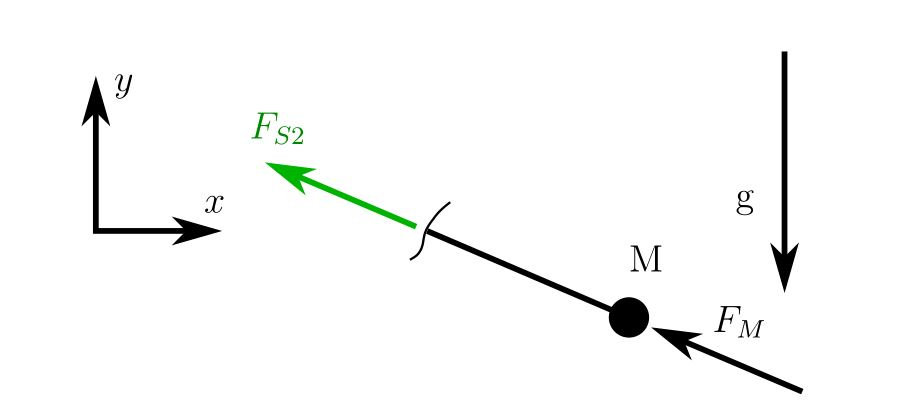
\includegraphics[width= 8cm]{tikz/13_07_2018_2h}
\end{figure}
\newline
Die Impulsbilanz ergibt mit der bekannten Geschwindigkeit
\[
	m_M\textbf{a}_M = \begin{bmatrix}
		F_{S2}\sin(\varphi_2) - F_M\sin(\varphi_2) \\
		F_{S2}\cos(\varphi_2) + F_M\cos(\varphi_2) - m_M
	\end{bmatrix}
\]
Durch Umformen dieser beiden Gleichungen, ergibt sich für die Stabkraft
\[
	F_{S2} = m_M\left(-a_{M,x}\sin(\varphi_2) + a_{M,y}\cos(\varphi_2)\right) - F_M + m_Mg\cos(\varphi_2)
\]